The aim of this text is to introduce the reader to topological dynamical systems and explore the various interpretations of chaos through the lens of topology and topological dynamical systems. A discrete dynamical system is defined by a metric space with a corresponding continuous function, mapping the metric space to itself. This function is termed a map or mapping whereby points in the underlying metric space are mapped to other points in the set by the application of this function. Topological dynamical systems themselves are a subset of discrete dynamical systems, with the extra requirement that the underlying metric space is compact (i.e.\ complete and totally bounded). This extra condition for compactness is useful for investigating the limiting behaviour of the set of iterates of the map as it is repeatedly iterated to infinity; a relevant feature in the study of chaos. The term chaos itself, specifically deterministic chaos, has various definitions in mathematics and was first coined by Li and Yorke in their ubiquitous paper `Period Three Implies Chaos' \cite{li-yorke}. Since then, a number of authors have proposed their own definitions of chaos, hinging on the existence of various properties of the topological dynamical system. The properties we shall be studying in this text include topological transitivity, the existence of a dense orbit, the density of periodic points, the existence of an uncountable scrambled set, sensitive dependence on initial conditions and topological entropy. Due to the differences between definitions of chaos, topological dynamical systems can be chaotic according to one interpretation but not another. We shall aim to compare these definitions and understand their consequences, providing examples of topological dynamical systems that exhibit each type of chaos. Specifically, we shall restrict our attention to four compact metric spaces: closed intervals, the unit circle, sequence space and compact countable sets; as these spaces have been heavily studied in literature. This text assumes the reader to be a capable student of pure mathematics with a basic understanding of topology and analysis. The focus of this text is mainly topological; for the sake of brevity content from related areas of ergodic theory, group theory, measure theory, etc.\ are excluded.

This chapter will briefly review some relevant results from topology before introducing ideas central to topological dynamics and the study of chaos in topological dynamical systems. We shall also introduce some popular topological dynamical systems that exhibit chaos, which we will be examining throughout this text. Subsequently, in Chapter \ref{chap:conjugacy-symbol-dynamics} we will introduce notions of comparing and equivalating topological dynamical systems using the framework of topological conjugacy and symbolic dynamics. Here we will use these powerful results to prove topological results for the well-known tent map and logistic map using a topological conjugacy. Furthermore, we shall begin our study of chaos via Sharkovsky's theorem. Finally, in Chapter \ref{chap:defining-chaos}, we will study the three various interpretations of chaos from called Devaney chaos, Li and Yorke chaos, and topological chaos, analysing examples of topological dynamical systems which satisfy each definition. We shall look at the various properties topological dynamical systems require to be considered chaotic and compare the various definitions.

\section{Topological Dynamical Systems and Discrete Dynamics} \label{sec:topological-dynamical-systems}
We shall start this chapter by giving the definition of a topological dynamical system, including some important definitions from topology and introducing some preliminary definitions from discrete dynamics. We shall refer back to these definitions constantly for the remainder of this text. Furthermore, prominent examples of topological dynamical systems will be presented. The reader should remember these examples as they will be integral to understanding several propositions in later chapters. Note that the definitions and results in this section apply generally to continuous maps, however, have been formulated in terms of topological dynamical systems for clarity and precision. Beginning, we shall introduce some preliminary definitions from topology.

\begin{defn}[Dense Set] \label{defn:dense}
    Let $(Z, d)$ be a metric space and $X, Y \subseteq Z$ where $X \subseteq Y$. The set $X$ is \emph{dense} in $Y$ if $\overline{X} = Y$, i.e.\ if for every $x \in Y$ there exists an open neighbourhood $U$ of $x$ with $y \in U$ such that $y \in X$.
\end{defn}

\begin{defn}[Finite Cover, Open Cover] \label{defn:cover}
    Let $(X, d)$ be a metric space. A \emph{finite cover} is a collection of sets $\mathcal{C} = \left\lbrace C_1, C_2, \dots, C_n \right\rbrace$ such that $X \subseteq \bigcup_{i = 1}^nC_i$. If the sets $C_1, C_2, \dots C_n$ are all open then $\mathcal{C}$ is a \emph{open cover}.
\end{defn}

\begin{defn}[Compact  Space] \label{defn:compact}
    A metric space $(X, d)$ is \emph{compact} if every open cover $\mathcal{U}$ of $X$ has a finite subcover $\left\lbrace U_{i(1)}, U_{i(2)}, \dots, U_{i(n)} \right\rbrace \subseteq \mathcal{U}$, i.e.\ if $\left\lbrace U_i \right\rbrace_{i\in I}$ is a collection of open subsets of $X$, where $X \subseteq \bigcup_{i \in I}U_i$ then there exists a finite subcollection $\left\lbrace U_{i(1)}, U_{i(2)}, \dots, U_{i(n)} \right\rbrace \subseteq \mathcal{U}$ such that $X \subseteq \bigcup_{j = 1}^{n}U_{i(j)}$. Furthermore, a metric space is compact if and only if it is complete and totally bounded.
\end{defn}

Note that on $\mathbb{R}$ with the standard metric, all closed intervals are compact. Since we now have a notion of what it means for a metric space to be compact, we can now define the main object we shall be studying in this paper, the topological dynamical system.

\begin{defn}[Topological Dynamical System] \label{defn:topological-dynamical-system}
    Let $X$ be a non-empty compact metric space. A \emph{topological dynamical system} denoted $(X, f)$ is given by a continuous map $f: X \to X$. The system starts at an initial point $x \in X$ and evolves through successive iterations of the map $f$. After $k \in \mathbb{N}$ iterations of $f$, the system can be described by $f^n := f \circ f \circ \dots \circ f$, where $x$ is mapped to the point $f^n(x)$. By convention we take $f^0$ to be the identity map.
\end{defn}

Having defined a topological dynamical system, we can now characterise the discrete dynamics of the underlying map through the following definitions.

\begin{defn}[Orbit] \label{defn:orbit}
    Let $(X, f)$ be a topological dynamical system. The \emph{orbit} or \emph{forward orbit} of a point $x \in X$ under $f$ is the set $\mathcal{O}_f(x) = \mathcal{O}^+_f(x) = \lbrace f^n(x) : n \geq 0 \rbrace = \lbrace x, f(x), f^2(x), \dots \rbrace$ of iterates of $x$ under the map $f$. If $f$ is a homeomorphism (i.e $f^{-1}$ exists and is continuous) then the \emph{backward orbit} of $x$ under $f$ is similarly defined as $\mathcal{O}^-_f(x) = \lbrace f^n(x) : n \leq 0 \rbrace = \lbrace x, f^{-1}(x), f^{-2}(x), \dots \rbrace$.
\end{defn}

Note that in this text, unless otherwise stated, the term, orbit, will simply refer to the forward orbit, as we will mostly be dealing with forward dynamics. An interesting characteristic which can occur in topological dynamical systems is the existence of a dense orbit. We shall explore various consequences that systems with this property hold in Chapter \ref{chap:defining-chaos}. For now, note that from Definition \ref{defn:dense} an orbit $\mathcal{O}_f(x)$ of $f$ is said to be dense in $X$ if for every $x \in X$ and $\varepsilon > 0$ there exists a $y \in X$ and $k \in \mathbb{N}$ such that $d(f^k(y), x) \leq \varepsilon$.

\begin{defn}[Periodic Point, Cycle] \label{defn:periodic-point}
    Let $(X, f)$ be a topological dynamical system. A point $x \in X$ is \emph{fixed} if $f(x) = x$ and \emph{periodic} if $f^n(x) = x$ for some $n \in \mathbb{N}$. The \emph{period} of a point $x$ is the least positive integer $k$ such that $f^k(x) = x$. If $x$ has a period of $k$ we say that $x$ is a \emph{period-$k$} point. The set of all period-$k$ points of $f$ is denoted by $\text{Per}_k(f)$ and the set of all periodic points of $f$ is denoted $\text{Per}(f)$. Moreover, $f^n(x) = x \iff n = lk$, for some $l \in \mathbb{N}$. The orbit $\mathcal{O}_f(x) = \lbrace x, f(x), \dots, f^{k-1}(x) \rbrace$ of a periodic point is a finite set of unique points, called a \emph{periodic orbit} of period $k$ or simply a \emph{k-cycle}.
\end{defn}

In most topological dynamical systems only a small subset of points are periodic. Most often a larger set of points either enter a periodic orbit after a certain number of iterations of $f$ or converge asymptotically to a periodic orbit, leading us directly into the following definitions.

\begin{defn}[Eventually Periodic, Asymptotically Periodic] \label{defn:eventually-asymptotically-periodic}
    Let $(X, f)$ be a topological dynamical system. A point $x \in X$ is \emph{eventually periodic} of period $k$ if the point $x$ is not periodic and there exists a $n > 0$ such that $f^{k+i}(x) = f^i(x)$, for $i \geq n$. The point $x \in X$ is \emph{asymptotically periodic} to a periodic point $p \in X$ if $\lim_{n \to \infty} d(f^n(x), f^n(p)) = 0$.
\end{defn}

\begin{prop} \label{prop:eventually-periodic-implies-periodic}
    Let $(X, f)$ be a topological dynamical system. If $f$ is an invertible map, then every eventually periodic point is periodic.
    \begin{proof}
        Suppose $x \in X$ is eventually periodic of period $k$ in $f$. Then $f^{k + i}(x) = f^i(x)$ for some $n > 0$. By applying $i$ iterations of $f^{-1}$ we obtain, $f^{-i} \circ f^{k + i}(x) = f^{-i} \circ f^{i}(x) \implies f^k(x) = x$. Hence $x$ is periodic with period $k$.
    \end{proof}
\end{prop}

When studying chaos in topological dynamical systems it can be useful to understand how the system behaves for an increasing number of iterations. The $\omega$-limit set, defined below as the set of limit points of a particular orbit, allows us to understand the behaviour of the system asymptotically.

\begin{defn}[Omega-limit Set] \label{defn:omega-limit-set}
    Let $(X, f)$ be a topological dynamical system. The $\omega$\emph{-limit} set of $x \in X$, denoted $\omega(x, f)$ is the set of all limit points of the orbit $\mathcal{O}_f(x)$ given by \[\omega(x, f) := \bigcap_{n=0}^\infty\overline{\left\lbrace f^k(x) : k \geq n \right\rbrace}\] and the $\omega$\emph{-limit} set of the entire map $f$ is defined as \[\omega(f) := \bigcup_{x \in X} \omega(x, f)\]
\end{defn}

By the definition, we can immediately see that the $\omega$-limit set of a period-$k$ point or eventually periodic point of period-$k$ is simply the $k$-cycle. Furthermore, if a point is asymptotically periodic then the $\omega$-limit set is clearly a cycle and hence finite. Now we are done with defining properties of discrete dynamics let's analyse the discrete dynamics of some popular topological dynamical systems.

\begin{exmp}[Logistic Map] \label{exmp:logitic-map}
    Define $F_{\mu}: [0, 1] \to [0, 1]$ to be the \emph{logistic map}, where $F_{\mu}(x)=\mu x(1-x)$ and $\mu > 0$. Since $[0, 1]$ is a closed interval it is compact. Hence $([0, 1], F_{\mu})$ describes a topological dynamical system.

    \begin{figure}[h]
        \centering
        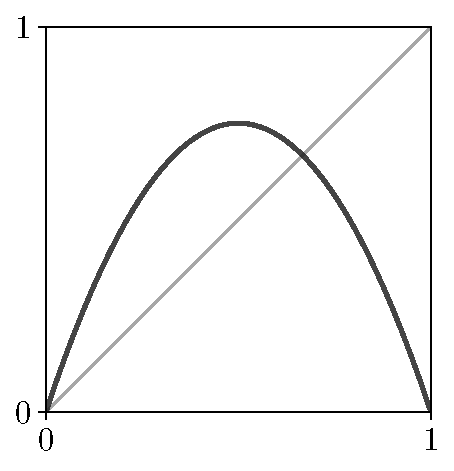
\includegraphics[width=4cm]{logistic_3}
        \caption{Logistic map $F_\mu$ with $\mu = 3$.}
        \label{fig:logistic_3}
    \end{figure}
\end{exmp}

\begin{exmp}[Tent Map] \label{exmp:tent-map}
    Define $T_s: [0, 1] \to [0,1]$ to be the \emph{tent map}, where $s \in (1, 2]$, $T_s(x) = sx$ for $x \in \left[0, \frac{1}{2}\right]$ and $T_s(x) = s(1-x)$ for $x \in \left[\frac{1}{2}, 1\right]$. Since $[0, 1]$ is a closed interval it is compact. Hence $([0, 1], T_s)$ describes a topological dynamical system. The dynamics of this system becomes difficult to understand as the number of iterations of $T_s$ increases due to the function's piecewise definition. In Chapter \ref{chap:conjugacy-symbol-dynamics} we shall develop the technique of using symbolic dynamics to better analyse the topological dynamics of this system.

    \begin{figure}[h]
        \centering
        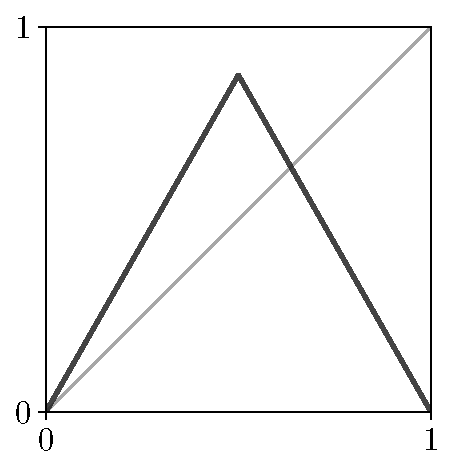
\includegraphics[width=4cm]{tent_1.75}
        \caption{Tent map $T_s$ with $s = \frac{7}{4}$.}
        \label{fig:tent_1.75}
    \end{figure}
\end{exmp}

\begin{exmp}[Doubling Map on $\left\lbrack 0, 1 \right\rbrack$] \label{exmp:doubling-map}
    Define $D: [0,1] \to [0,1]$ to be the \emph{doubling map on} $[0, 1]$, where $D(x) = 2x$ for $x \in \left[0, \frac{1}{2}\right]$ and $D(x) = 2x - 1$ for $x \in \left[\frac{1}{2}, 1\right]$. Since $[0, 1]$ is a closed interval it is compact. However, the map $D$ is not continuous as a discontinuity exists at $x = \frac{1}{2}$ and so this is not a dynamical system, however, we shall use this maps properties to establish results about other topological dynamical systems. Just like the tent map, the dynamics of this system become difficult to understand as the number of iterations of $D$ increases.

    \begin{figure}[h]
        \centering
        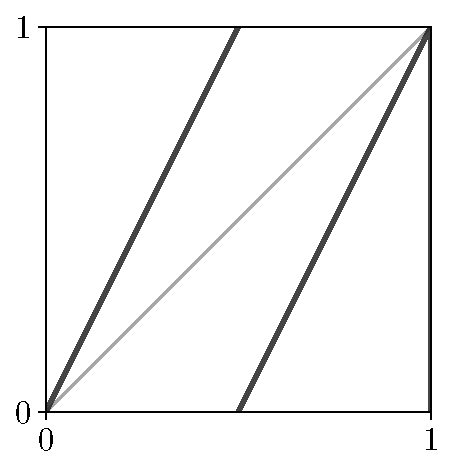
\includegraphics[width=4cm]{doubling}
        \caption{Doubling map $D$.}
        \label{fig:doubling}
    \end{figure}
\end{exmp}

Note that throughout this text we shall define $S^1 = \left\lbrace z \in \mathbb{C}: |z| = 1 \right\rbrace = \left\lbrace e^{i\theta} : 0 \leq \theta \leq 2\pi \right\rbrace$ and is the unit circle in the complex plane. The metric space $(S^1, d)$ is defined using the arc length metric, where $d(x, y)$ is the shortest arc connecting $x$ to $y$. 

\begin{exmp}[Doubling Map on $S^1$] \label{exmp:doubling-map-s1}
    Define $\mathcal{D}: S^1 \to S^1$ to be the \emph{doubling map on} $S^1$, where $\mathcal{D}(z) = z^2$, or equivalently $\mathcal{D}(e^{i\theta}) = e^{2i\theta}$ for some $\theta \in \mathbb{R}$.

    \begin{figure}[h]
        \centering
        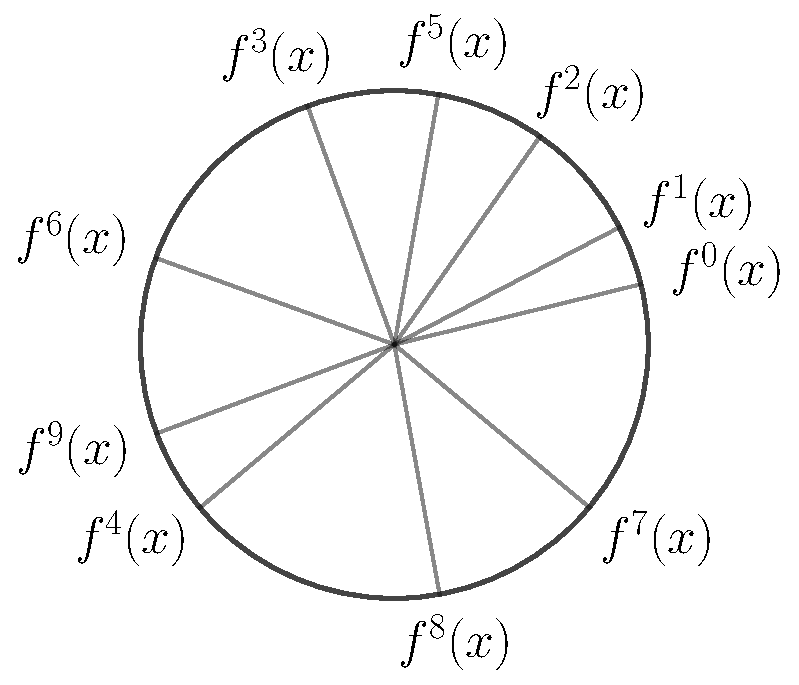
\includegraphics[width=5cm]{doubling_circle}
        \caption{First ten iterations of the doubling map $\mathcal{D}$.}
        \label{fig:doubling-circle}
    \end{figure}
\end{exmp}

\begin{exmp}[Rigid Rotations] \label{exmp:rigid-rotations}
    Define $R_\alpha: S^1 \to S^1$ to be the \emph{rigid rotations of the unit circle}, where $\alpha \in [0, 2\pi)$ and the function $R_{\alpha}(z) = ze^{i\alpha}$, or equivalently $R_\alpha(e^{i\theta}) = e^{i(\theta + \alpha)}$. Note that $S^1$ is compact as it is a closed subset of $\mathbb{R}$. Hence $(S^1, R_{\alpha})$ describes a topological dynamical system.

    \begin{figure}[h]
        \centering
        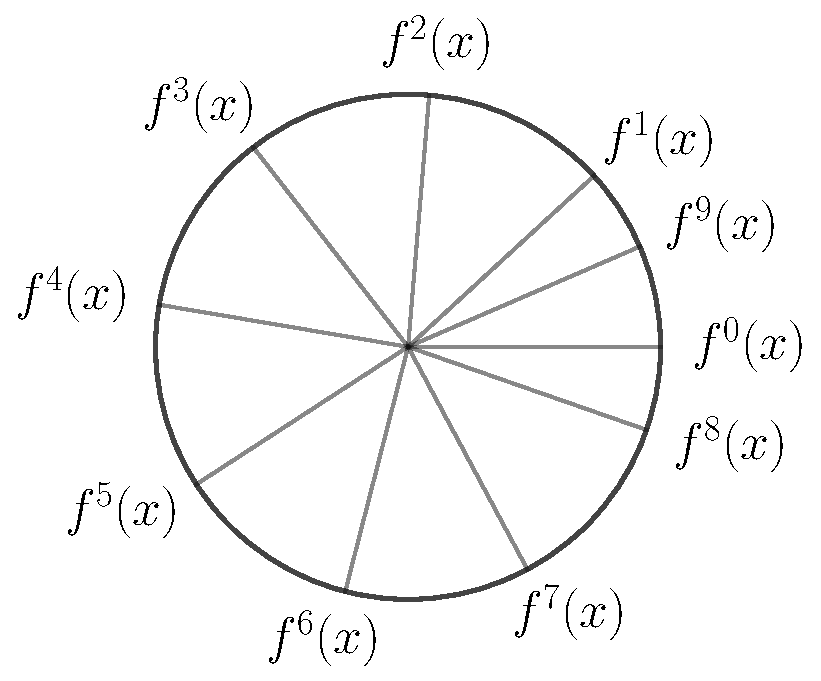
\includegraphics[width=5cm]{rigid_circle}
        \caption{First ten iterations of the rigid rotations $R_\alpha$.}
        \label{fig:rigid-circle}
    \end{figure}
\end{exmp}

An interesting property of the rigid rotations is how the behaviour of the dynamical system changes depending on the rationality or irrationality of $\alpha$. This brings us to the following proposition.

\begin{prop} \label{prop:rigid-rotations-irrational}
    If $\alpha$ is an irrational number, then for all $z \in S^1$, the orbit $\mathcal{O}_{R_\alpha}(z)$ is infinite and dense on $S^1$.
    \begin{proof}
        Let $z \in S^1$ be arbitrary. If $R_\alpha^m(z) = R_\alpha^n(z)$ for some $m, n \in \mathbb{Z}$ then $ze^{(m-n)i\alpha} = z \implies (m - n)i\alpha = 0$. Since $\alpha \notin \mathbb{Q}$ and $(m - n)\alpha \neq 2\pi n$ for $n \in \mathbb{N}$ we have $m = n$. Hence all the points in the orbit are distinct and so $\mathcal{O}_{R_\alpha}(z)$ is infinite. Now let $w \in S^1$ be arbitrary and let $\varepsilon > 0$. Choose $N$ such that $\frac{2\pi}{N} < \varepsilon$. Now there exists $0 \leq l, k \leq N$ such that $d\left( R_\alpha^k, R_\alpha^l \right) \leq \frac{2\pi}{N}$. As $R_\alpha$ is an isometry i.e. $d(R_\alpha(x), R_\alpha(y)) = d(x, y)$ we obtain $d(R_\alpha^{(k - l)}(z), z) \leq \varepsilon$. Now since $R_\alpha$ is an isometry, the set $X = \lbrace R_\alpha^{n(k - l)}(z) : n \in \mathbb{N} \rbrace$ partitions $S^1$ into arcs of of length less than $\varepsilon$. Hence there must exist a $R_\alpha^{i(k - l)}(z) \in X$ such that $d(R_\alpha^{i(k - l)}(z), w) \leq \varepsilon$ and so $\mathcal{O}_{R_{\alpha}}$(z) is dense on $S^1$.
    \end{proof}
\end{prop}

Depending on the parameters $s$, $\mu$ and $\alpha$ the dynamical behaviour of these systems can range from predictable periodicity to chaotic. In Chapter \ref{chap:conjugacy-symbol-dynamics} we shall subsequently prove that $T_2$ and $F_4$ are similar topologically speaking and share various topological properties. Moreover, both of these topological dynamical systems are described by simple mathematical equations, however, we shall prove later that they are chaotic and exhibit highly complex and irregular dynamics.